% !TeX root = ../FinalRepordCS.tex

\chapter{System modeling and structure}

\section{Communication Architecture}

The architecture mainly describes Alice and Bob as two LoRa nodes that need to generate the same communication key. It starts with one of them initiating the key generation communication (a random LoRa message with a sequence number). When the other party (Bob) receives the request, it immediately replies with a message with a sequence number.
The pair of two LoRa packets that in the communicate with each other are both marked with RSSI. These tags are mainly generated by the strength of the signal via the communication. Since wireless message transmission can be regarded as extremely fast propagation, which is close to the speed of light, the RSSI values that the two nodes can obtain in this communication process are close. Or, to be more specific, if LoRa messages are generated with the same pattern, the trend of RSSI values obtained at both ends over a period of time is close.
In addition, since RSSI is mainly affected by signal strength, in the real world, it is generally due to changes in the surrounding environment, such as changes in the communication distance between the two nodes, the appearance of some obstacles between the nodes, the weather, or interference from other signals, etc. For the two nodes, the impact is the same, especially for the physical communication channel formed by the two nodes. Therefore, the trend of RSSI values obtained by the two nodes is a good physical layer feature factor.
\begin{figure}
  \centering
  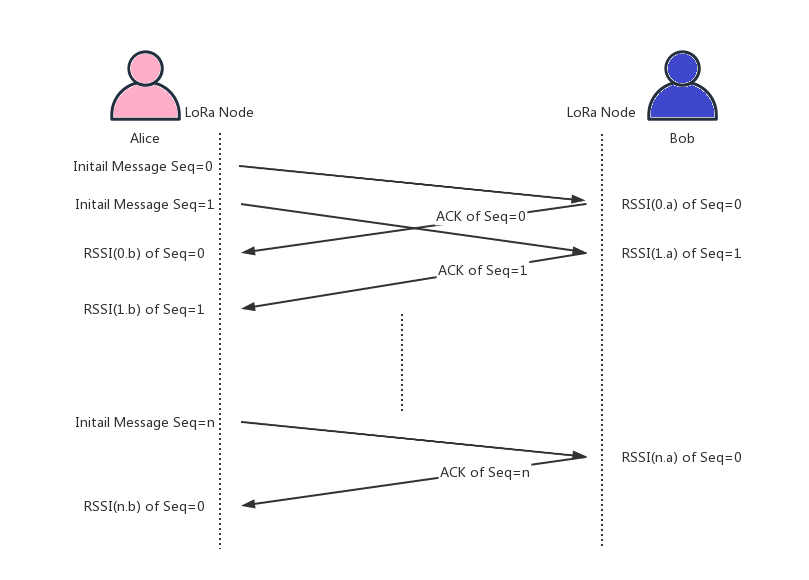
\includegraphics[width=0.7\linewidth]{fig4-1.png}
  \caption{Communication Architecture}
  \label{fig:4-1}
\end{figure}
As shown in the figure 4-1, after $n$ interactions, $n$ pairs of RSSI values can be obtained. Then, through a certain algorithm, the $n$ pairs of RSSI values can be modulated and used as factors to generate a key. In this way, the two nodes can obtain a common physical layer communication key. 
However, in actual use, due to interference from the actual environment, such as physical obstruction, channel blocking, and frequency band interference, the LoRa communication packets cannot always be received as expected. In particular, due to long-distance transmission, LoRa physical layer messages are not reliable transmissions, so packet loss needs to be considered. In addition, according to this communication model, the biggest challenge to generating a pair of RSSI is still Bob's reply message. This is because Bob's reply is based on the premise of receiving Alice's message, but Alice may not be able to receive Bob's reply.

\section{LoRa End Nodes Modeling and Algorithm}
As mentioned in the previous text, LoRa nodes are half-duplex devices. In order to implement the mentioned functional model, a specific algorithm is required to enable LoRa nodes to both listen to messages and transmit messages after receiving information.
One way to implement this functional model is to use a polling approach. In this approach, LoRa nodes periodically poll other nodes to see if they have any information to send. If the polling detects that other nodes have information to send, the LoRa node will stop listening and transmit a message.Another way to implement this functional model is to use an event-driven approach. In this approach, LoRa nodes register an event handler that will be triggered when they receive information from other nodes. When the event handler is triggered, the LoRa node will stop listening and transmit a message.
Specifically, in the polling approach, LoRa nodes can use the following steps to implement the aforementioned functional model:
\begin{itemize}
  \item Set a polling interval, such as 100 milliseconds.
  \item Within the polling interval, LoRa nodes will send a query message to other nodes.
\end{itemize}
If LoRa nodes receive a response message from other nodes, the LoRa nodes will stop listening and transmit a message.
In the event-driven approach, LoRa nodes can use the following steps to implement the aforementioned functional model:
\begin{itemize}
  \item Register an event handler that will be triggered when they receive information from other nodes.
  \item In the event handler, LoRa nodes will stop listening and transmit a message.
\end{itemize}
Both of these algorithms have their own advantages and disadvantages. The advantage of the polling approach is that it is simple to implement, but it can reduce the LoRa node's receiving sensitivity. The advantage of the event-driven approach is that it can improve the LoRa node's receiving sensitivity, but it requires additional overhead for the event handler.
\begin{algorithm}[hbt!]
  \caption{Algorithm for Alice}\label{alg:Alice}
  \begin{algorithmic}
  \State Initialize variables:
      \State $lastSendTime \gets 0$
      \State $interval \gets$ user-defined interval
      
      \Function{loop}{}
          \If{$\text{millis()} - \text{lastSendTime} > \text{interval}$}
              \State $message \gets \text{"SEQ"} \gets n$
              \State \Call{sendMessage}{$message$}
              \State \textbf{print} "Sending" $+$ $message$
              \State $lastSendTime \gets \text{millis()}$
              \State $interval \gets \text{random}(2000) + 1000$ \Comment{2-3 seconds}
          \EndIf
          \State \textbf{parse for a packet, and call} \Call{onReceive}{\text{parsePacket()}}
      \EndFunction
  \end{algorithmic}
\end{algorithm}
The purpose of this algorithm is to establish a two-way communication channel over LoRa. The “SEQ” message is a special message that is used to initiate a communication session. The onReceive() function can be used to process any incoming messages, such as acknowledgment messages or data messages.
The loop starts by checking the millis() function to see how long it has been since the last message was sent. If it has been longer than the interval period, then the loop sends a SYN message using the sendMessage() function.
The loop then calls the onReceive() function to parse for any incoming packets. If a packet is received, the onReceive() function will be called with the parsed packet data.
\begin{algorithm}[hbt!]
  \caption{Algorithm for sendMessage}\label{alg:sendMessage}
  \begin{algorithmic}
  \Function{sendMessage}{$\text{outgoing}$}
          \State Initialize $message$
          \State Add $message \gets \text{Payload} \gets outgoing$
          \State Send $message$
          \State $msgCount \gets$ $msgCount + 1$
      \EndFunction
  \end{algorithmic}
  \end{algorithm}
The sendMessage algorithm encapsulates a message for LoRa communication. It constructs a packet containing destination and sender addresses, a message ID, payload length, and the actual message. The LoRa packet is then sent, and the message ID is incremented for the next message. This function is designed for a larger program implementing LoRa communication.
  \begin{algorithm}[hbt!]
    \caption{onReceive Algorithm for Alice}\label{alg:onReceive}
    \begin{algorithmic}
        \Function{onReceive}{$\text{packetSize}$}
            \If{$\text{packetSize} = 0$}
                \State \textbf{return}
            \EndIf
            \State \Comment{Read packet header bytes:}
            \State Initialize $incoming$ 
            \While{\text{LoRa.available()}}
                \State $incoming \gets incoming + (\text{char})\text{LoRa.read()}$
            \EndWhile
            
            \If{$\text{incomingLength} \neq \text{incoming.length()}$}
                \State \textbf{print} "error: message length does not match length"
                \State \textbf{return}
            \EndIf
            
            \If{$recipient \neq \text{localAddress} \land recipient \neq 0xFF$}
                \State \textbf{print} "This message is not for me."
                \State \textbf{return}
            \EndIf
            
            \State \Comment{Print message details for this device or broadcast:}
            \State \textbf{print} $message$
        \EndFunction
    \end{algorithmic}
\end{algorithm}
The onReceive algorithm for Alice processes incoming LoRa packets, extracting and verifying header information, checking the recipient address, and providing detailed information about the received message, including sender and recipient addresses, message ID, length, RSSI values, and Snr.
\begin{algorithm}[hbt!]
  \caption{Algorithm for Bob}\label{alg:Bob}
  \begin{algorithmic}
  \State Initialize variables
      
      \Function{loop}{}
          \State \textbf{parse for a packet, and call} \Call{onReceive}{\text{parsePacket()}}
      \EndFunction
  \end{algorithmic}
\end{algorithm}
The algorithm for bob continuously parses for incoming LoRa packets and invokes the onReceive function, passing the result of as the packet size parameter.
\begin{algorithm}[hbt!]
  \caption{onReceive Algorithm for Bob}\label{alg:BobonReceive}
  \begin{algorithmic}
      \Function{onReceive}{$\text{packetSize}$}
          \State Algorithm 4.3 onReceive Algorithm for Alice
          \State $outgoing \gets incoming.SEQ$
          \State \textbf{print} $sendMessage(outgoing)$
      \EndFunction
  \end{algorithmic}
\end{algorithm}
The onReceive algorithm for Bob processes incoming LoRa packets, extracting and verifying header information, checking the recipient address, providing detailed information about the received message, and then sending a response message containing the received signal strength indication (RSSI) using the sendMessage function.

\section{Physical Layer Key Generation Modeling and Algorithm}
After the LoRa end node setup, we can process the physical layer key generation by the following steps:
\begin{algorithm}[hbt!]
  \caption{RSSI-Based Key Generation Algorithm}\label{alg:keygeneration}
  \begin{algorithmic}
  
  \Require $X_A$ and $X_B$ :  the original sample RSSI list
  
  \State Initialize variables
  
  \State $X_A'$, $X_B'$ $\gets$ Savitzky–Golay filter($X_A$, $X_B$)
  \Repeat
      \State $K_A'$ $\gets$ Quantization($X_A'$)
      \State $K_B'$ $\gets$ Quantization($X_B'$)
  \Until{$K_A'' \gets Reconciliation(K_A') = K_B'$}
  
  \State $K_{Share} \gets$ Privacy\_Amplification($K_A''$, $K_B'$)
  
  \State \Return $K_{Share}$ \Comment{Secret Key for Alice and Bob}
  
  \end{algorithmic}
\end{algorithm}

\textbf{Sampling:} Alice and Bob exchange a number of probe and response packets to sample the RSSI channel by the mentioned in 4.2 LoRa End Nodes Modeling and Algorithm.

\textbf{Signal processing:} Alice and Bob apply outlier detection and Savitzky–Golay filter, which is mentioned in 3.2.5, to reduce the discrepancies caused by the environmental noise. They then use linear interpolation to construct missing data points. The Savitzky–Golay algorithm is a method for smoothing and differentiating data. Given a set of data points \(y_i\) at positions \(x_i\) for \(i = 1, 2, \ldots, n\), the smoothed data \(\hat{y}_i\) is computed using the convolution operation:
\begin{equation}
\hat{y}_i = \sum_{j = -k}^{k} c_j \cdot y_{i+j}
\end{equation}
where \(k\) is the half-width of the smoothing window and \(c_j\) are the Savitzky–Golay coefficients. The coefficients can be computed by solving the linear system of equations:
\begin{equation}
\begin{bmatrix}
  S_0 & S_1 & \ldots & S_{2k} \\
  S_1 & S_2 & \ldots & S_{2k+1} \\
  \vdots & \vdots & \ddots & \vdots \\
  S_{2k} & S_{2k+1} & \ldots & S_{4k}
\end{bmatrix}
\begin{bmatrix}
  c_{-k} \\
  c_{-(k-1)} \\
  \vdots \\
  c_k
\end{bmatrix}
=
\begin{bmatrix}
  0 \\
  0 \\
  \vdots \\
  1
\end{bmatrix}
\end{equation}
where \(S_j = \sum_{i=1}^{n} x_i^j\). The solution to this system provides the coefficients \(c_j\) for the convolution operation.

\textbf{Multilevel Quantization:} Alice and Bob convert the RSSI values to bit strings by employing multilevel quantization technique.
\begin{algorithm}[hbt!]
  \caption{Multilevel Quantization}\label{alg:Quantization}
  \begin{algorithmic}
  \Function{Quantization}{$\text{sampleArray}, \text{numBitsPerSample}, \text{alpha}$}
      \State $Variables\ Initailzation$
  
      \For{$i \gets 1$ \textbf{to} $M$}
          \State $\text{levelBase}[i] \gets \text{offset}$
          \State $\text{levelTop}[i] \gets \text{levelBase}[i] + \text{stepSize}$
          \State $\text{offset} \gets \text{offset} + \text{stepSize} + \text{gbandSize}$
      \EndFor
  
      \State $\text{decimalValArray} \gets []$
      \State $\text{validIndices} \gets []$
  
      \For{$i \gets 1$ \textbf{to} $\text{sampleArrayLength}$}
          \For{$j \gets 1$ \textbf{to} $M$}
              \If{$\text{sampleArray}[i] = \text{minVal}$}
                  \State $\text{decimalValArray}[i] \gets 1$ \Comment{Decimal assignment starts from 0}
                  \State $\text{validIndices}[i] \gets i$
                  \State \textbf{break}
              \ElsIf{$\text{sampleArray}[i] = \text{maxVal}$}
                  \State $\text{decimalValArray}[i] \gets M - 1$ 
                  \State $\text{validIndices}[i] \gets i$
                  \State \textbf{break}
              \ElsIf{$\text{levelBase}[j - 1] \leq \text{sampleArray}[i] \leq \text{levelTop}[j - 1]$}
                  \State $\text{decimalValArray}[i] \gets j - 1$ 
                  \State $\text{validIndices}[i] \gets i$
                  \State \textbf{break}
              \EndIf
          \EndFor
      \EndFor
  
      \State $Variables\ Updating$
  
      \For{$i \gets 1$ \textbf{to} $\text{decimalValArrayLen}$}
          \State $\text{bitString}.\text{extend}(\text{format}(\text{decimalValArray}[i], \text{f}'0\{\text{numBitsPerSample}\}b'))$
      \EndFor
  
      \State \Return $\text{bitString}, \text{validIndices}$
  \EndFunction
  \end{algorithmic}
\end{algorithm}

The function uses M-ary quantization to represent the input samples with a specified number of bits per sample, considering guard bands to reduce quantization errors. The resulting bit string can be used for further processing or transmission.

\textbf{Reconciliation:} Alice and Bob use a CS-based reconciliation method to correct the bit mismatches between their bit strings.
\begin{algorithm}[hbt!]
  \caption{Reconciliation Algorithm}\label{alg:Reconciliation}
  \begin{algorithmic}
  \Function{Reconciliation}{$A, y$}
      \State $Variables\ Initailzation$
  
      \For{$\text{iter\_idx} \gets 1$ \textbf{to} $\text{iter\_times}$}
          \State $\text{c} \gets A^T \cdot (y - A \cdot x)$
          \State $\text{lambda\_max\_idx} \gets \text{argmax}(|\text{c}|)$
          \State $\text{lambda\_max} \gets |\text{c}[\text{lambda\_max\_idx}]|$
  
          \State $\text{act\_set} \gets \text{where}(|\text{c} - \text{lambda\_max}| < 1e-5)$
  
          \State $\text{state} \gets \text{zeros vector of size } m$
          \State $\text{state}[\text{act\_set}] \gets 1$
  
          \State $R \gets A[:, \text{act\_set}]^T \cdot A[:, \text{act\_set}]$
          \State $d \gets \text{pinv}(R) \cdot \text{sign}(c[\text{act\_set}])$
  
          \State $\text{gamma} \gets 1000$
  
          \For{$\text{idx} \gets 1$ \textbf{to} $m-1$}
              \If{$\text{state}[\text{idx}]$}
                  \State $\text{my\_id} \gets \text{where}(\text{act\_set} = \text{idx})$
                  \State $\text{tmp} \gets \max(0, -x[\text{idx}] / d[\text{my\_id}])$
              \Else
                  \State $\text{av} \gets A[:, \text{idx}]^T \cdot (A[:, \text{act\_set}] \cdot d)$
                  \State $\text{tmp1} \gets \max(0, (\text{lambda\_max} - c[\text{idx}]) / (1 - \text{av}))$
                  \State $\text{tmp2} \gets \max(0, (\text{lambda\_max} + c[\text{idx}]) / (1 + \text{av}))$
                  \State $\text{tmp} \gets \min(\text{tmp1}, \text{tmp2})$
              \EndIf
  
              \If{$\text{tmp} > 0$}
                  \State $\text{gamma} \gets \min(\text{tmp}, \text{gamma})$
              \EndIf
          \EndFor
  
          \State $x[\text{act\_set}] \gets x[\text{act\_set}] + (\text{gamma} \cdot d)[0]$
  
          \If{$\|y - A \cdot x\|_2 < 1e-6$}
              \State \textbf{break}
          \EndIf
      \EndFor
  
      \State \Return $x, \text{iter\_idx}$
  \EndFunction
  \end{algorithmic}
  \end{algorithm}
The Reconciliation algorithm is commonly used for solving sparse linear regression problems, where the $l1$ regularization encourages sparsity in the solution. The function iteratively refines the solution by updating the active set and adjusting the solution vector based on the direction and step size. The algorithm terminates when the convergence criterion is satisfied or after a specified number of iterations.
The algorithm then computes the active set, which is the set of indices of the elements in the solution that have the largest residual correlations. The active set is computed by finding the elements in the solution that have a residual correlation that is within $1e-5$ of the maximum residual correlation.
After Reconciliation, performs computing the bitwise exclusive-Or (XOR) of two binary arrays, \textbf{bits\_a} (Bits of Alice after Quantization) and mismatch, and then casting the result to an integer array. This is a useful operation for error correction, as it can be used to recover the original bits from a corrupted set of bits, provided that the number of errors is less than half the number of bits. 
  \[
  \text{{bits\_recover}} = \text{{np.logical\_xor}}(\textbf{\framebox[1.1\width]{{bits\_a}}}, \text{{mismatch}}.\text{{reshape}}(\text{{len}}(\text{{mismatch}}))).\text{{astype(int)}}
  \]
\textbf{Key Extraction:} Alice and Bob extract a secure key from the reconciled bit strings using a shared secret key or a one-way hash function. Considering that the computing power of LoRa nodes is limited, especially in the case of IoT nodes without AES hardware acceleration, Chacha20(RFC 7539)\cite{rfc7539}, a symmetric encryption algorithm that is more suitable for embedded hardware, is chosen here. ChaCha20-Poly1305 has a simpler process than the traditional AES algorithm and has achieved better performance such that in the absence of a dedicated accelerator\cite{7507408,7927078}.
\begin{algorithm}
    \caption{ChaCha20-Poly1305 Encryption}
    \begin{algorithmic}[1]
    \Function{ChaCha20Poly1305Encrypt}{$\text{plaintext}, \text{key}, \text{nonce}$}
        \State $\text{ciphertext} \gets \text{ChaCha20}(\text{plaintext}, \text{key}, \text{nonce})$
        \State $\text{tag} \gets \text{Poly1305}(\text{ciphertext}, \text{key})$
        \State \Return $\text{ciphertext}, \text{tag}$
    \EndFunction
    \end{algorithmic}
\end{algorithm}
    
    \begin{algorithm}
    \caption{ChaCha20-Poly1305 Decryption}
    \begin{algorithmic}[1]
    \Function{ChaCha20Poly1305Decrypt}{$\text{ciphertext}, \text{key}, \text{nonce}, \text{tag}$}
        \State $\text{plaintext} \gets \text{ChaCha20}(\text{ciphertext}, \text{key}, \text{nonce})$
        \State $\text{computedTag} \gets \text{Poly1305}(\text{ciphertext}, \text{key})$
        \If{$\text{computedTag} \neq \text{tag}$}
            \State \textbf{throw} AuthenticationError
        \EndIf
        \State \Return $\text{plaintext}$
    \EndFunction
    \end{algorithmic}
\end{algorithm}